% Preámbulo
\documentclass[letterpaper]{article}
\usepackage[utf8]{inputenc}
\usepackage[spanish]{babel}

\usepackage{enumitem}
\usepackage{titling}

% Símbolos
	\usepackage{amsmath}
	\usepackage{amssymb}
	\usepackage{amsthm}
	\usepackage{amsfonts}
	\usepackage{mathtools}
	\usepackage{bbm}
	\usepackage[thinc]{esdiff}
	\allowdisplaybreaks

% Márgenes
	\usepackage
	[
		margin = 1.2in
	]
	{geometry}

% Imágenes
	\usepackage{float}
	\usepackage{graphicx}
	\graphicspath{{imagenes/}}
	\usepackage{subcaption}

% Ambientes
	\usepackage{amsthm}

	\theoremstyle{definition}
	\newtheorem{ejercicio}{Ejercicio}

	\newtheoremstyle{lemathm}{4pt}{0pt}{\itshape}{0pt}{\bfseries}{ --}{ }{\thmname{#1}\thmnumber{ #2}\thmnote{ (#3)}}
	\theoremstyle{lemathm}
	\newtheorem{lema}{Lema}

	\newtheoremstyle{lemathm}{4pt}{0pt}{\itshape}{0pt}{\bfseries}{ --}{ }{\thmname{#1}\thmnumber{ #2}\thmnote{ (#3)}}
	\theoremstyle{lemathm}
	\newtheorem{sol}{Solución}
	
	\newtheoremstyle{lemathm}{4pt}{0pt}{\itshape}{0pt}{\bfseries}{ --}{ }{\thmname{#1}\thmnumber{ #2}\thmnote{ (#3)}}
	\theoremstyle{lemathm}
	\newtheorem{theo}{Teorema}

	\newtheoremstyle{lemademthm}{0pt}{10pt}{\itshape}{ }{\mdseries}{ --}{ }{\thmname{#1}\thmnumber{ #2}\thmnote{ (#3)}}
	\theoremstyle{lemademthm}
	\newtheorem*{lemadem}{Demostración}

% Macros
	\newcommand{\sumi}[2]{\sum_{i=#1}^{#2}}
	\newcommand{\dint}[2]{\displaystyle\int_{#1}^{#2}}
	\newcommand{\inte}[2]{\int_{#1}^{#2}}
	\newcommand{\dlim}{\displaystyle\lim}
	\newcommand{\limxinf}{\lim_{x\to\infty}}
	\newcommand{\limninf}{\lim_{n\to\infty}}
	\newcommand{\dlimninf}{\displaystyle\lim_{n\to\infty}}
	\newcommand{\limh}{\lim_{h\to0}}
	\newcommand{\ddx}{\dfrac{d}{dx}}
	\newcommand{\txty}{\text{ y }}
	\newcommand{\txto}{\text{ o }}
	\newcommand{\Txty}{\quad\text{y}\quad}
	\newcommand{\Txto}{\quad\text{o}\quad}
	\newcommand{\si}{\text{si}\quad}

	\newcommand{\etiqueta}{\stepcounter{equation}\tag{\theequation}}
	\newcommand{\tq}{:}
	\renewcommand{\o}{\circ}
	\newcommand*{\QES}{\hfill\ensuremath{\blacksquare}}
	\newcommand*{\qes}{\hfill\ensuremath{\square}}
	\newcommand*{\QESHERE}{\tag*{$\blacksquare$}}
	\newcommand*{\qeshere}{\tag*{$\square$}}
	\newcommand*{\QED}{\hfill\ensuremath{\blacksquare}}
	\newcommand*{\QEDHERE}{\tag*{$\blacksquare$}}
	\newcommand*{\qel}{\hfill\ensuremath{\boxdot}}
	\newcommand*{\qelhere}{\tag*{$\boxdot$}}
	\renewcommand*{\qedhere}{\tag*{$\square$}}

	\newcommand{\suc}[1]{\left(#1_n\right)_{n\in\N}}
	\newcommand{\en}[2]{\binom{#1}{#2}}
	\newcommand{\upsum}[2]{U(#1,#2)}
	\newcommand{\lowsum}[2]{L(#1,#2)}
	\newcommand{\abs}[1]{\left| #1 \right| }
	\newcommand{\bars}[1]{\left \| #1 \right \| }
	\newcommand{\pars}[1]{\left( #1 \right) }
	\newcommand{\bracs}[1]{\left[ #1 \right] }
	\newcommand{\inprod}[1]{\left\langle #1 \right\rangle }
        \newcommand{\norm}[1]{\left\lVert#1\right\rVert}
        \newcommand{\floor}[1]{\left \lfloor #1 \right\rfloor }
	\newcommand{\ceil}[1]{\left \lceil #1 \right\rceil }
	\newcommand{\angles}[1]{\left \langle #1 \right\rangle }
	\newcommand{\set}[1]{\left \{ #1 \right\} }
	\newcommand{\norma}[2]{\left\| #1 \right\|_{#2} }


	\newcommand{\NN}{\mathbb{N}}
	\newcommand{\QQ}{\mathbb{Q}}
	\newcommand{\RR}{\mathbb{R}}
	\newcommand{\ZZ}{\mathbb{Z}}
	\newcommand{\PP}{\mathbb{P}}
        \newcommand{\EE}{\mathbb{E}}
	\newcommand{\1}{\mathbbm{1}}
	\newcommand{\eps}{\varepsilon}
	\newcommand{\ttF}{\mathtt{F}}
	\newcommand{\bfF}{\mathbf{F}}

	\newcommand{\To}{\longrightarrow}
	\newcommand{\mTo}{\longmapsto}
	\newcommand{\ssi}{\Longleftrightarrow}
	\newcommand{\sii}{\Leftrightarrow}
	\newcommand{\then}{\Rightarrow}

	\newcommand{\pTFC}{{\itshape 1er TFC\/}}
	\newcommand{\sTFC}{{\itshape 2do TFC\/}}


% Datos
    \title{Análisis de Algoritmos e introducción a Matemáticas Discretas \\ Tarea 1}
    \author{Rubén Pérez Palacios Lic. Computación Matemática\\Profesor: Dr. Carlos Segura González}
    \date{\today}

% DOCUMENTO
\begin{document}
	\maketitle

    \begin{enumerate}[label=\textbf{Problema \arabic*}]
        \item \textbf{(2 puntos).} En las sesiones de clases, se explicó que cuando en el vector de la stl se hace un push\_back, y no hay memoria suficiente para albergar otro elemento, se pide memoria adicional, y se procede a copiar todos los elementos que ya se tenían en el vector a las nuevas posiciones de memoria. Supongamos que inicialmente tenemos un vector vacío, con espacio reservado para un elemento, y que se van a realizar $n = 2^p$ inserciones.
        
        \begin{enumerate}
            \item Determine el número de escrituras en memoria que se realizarán si cada vez que el vector se queda sin memoria, se pide memoria para un espacio adicional. Especifique el número de escrituras $e\pars{n}$ de forma exacta, grafíquelo, y encuentre una función $g\pars{n}$ lo más simple posible, de forma que $e\pars{n} = \Theta\pars{g\pars{n}}$.
            
			Debido a que cada vez que se agrega un elemento al vector se copia todo el vector a otro vector cuyo tamaño crece en 1, entonces al insertar el $i-esimo$ elemento se harán $i$ escrituras, por lo tanto el número de escrituras en memoria que se realizarán son $e\pars{n} = \sum_{i=1}^n i = \frac{\pars{n}\pars{n+1}}{2} = \frac{\pars{2^{p}}\pars{2^{p}+1}}{2}$, la cual es $e\pars{n} = \Theta(n^{2}) = \Theta(4^{p})$ y cuya gráfica es:

			\begin{figure}[H]
				\begin{center}
					\includegraphics[scale=0.8]{Images/Agregando de uno en uno.png}
				\end{center}
			\end{figure}

			
            \item Determine el número de escrituras en memoria que se realizarán si cada vez que el vector se queda sin memoria, se duplica la cantidad de espacio reservado. Especifique el número de escrituras $e\pars{n}$ de forma exacta, grafíquelo, y encuentre una función $g\pars{n}$ lo más simple posible, de forma que $e\pars{n} = \theta\pars{g\pars{n}}$.
            
			Primero para cada elemento que se inserte se tenga que aumentar el tamaño o no del vector tendras que escribir este, por lo que se harán al menos $n$ acciones. Ahora el vector necesitara aumentar su tamaño cada que se inserte un $i-esimo$ elemento donde $i$ es de la forma $2^k + 1$ para algún $k$ entero, y en cada una de estas se harán $2^k$ escrituras por lo que el total de escrituras para las copias es de $\sum_{i=0}^{p-1} 2^i = 2^{p}-1 = n-1$. Por lo tanto el número de escrituras en memoria que se realizarán son $e\pars{n} = 2n-1$, la cual es $e\pars{n} = \Theta(n)$ y cuya gráfica es:
			
			\begin{figure}[H]
				\begin{center}
					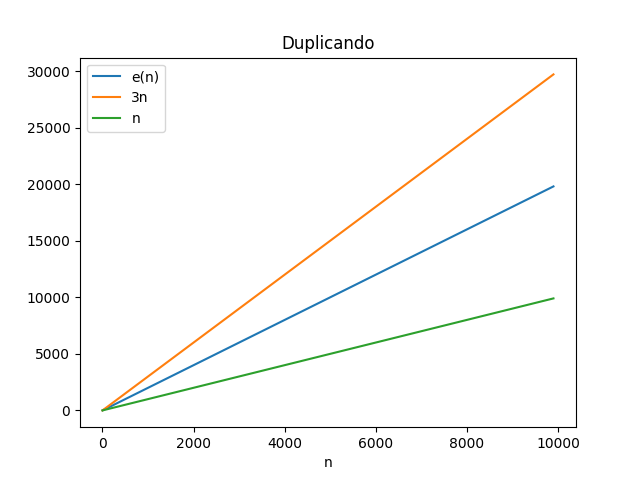
\includegraphics[scale=0.80]{Images/Duplicando.png}
				\end{center}
			\end{figure}
			
			\newpage

            \item Determine el número de escrituras en memoria que se realizarán si cada vez que el vector se queda sin memoria, se multiplica por 4 la cantidad de espacio. Especifique el número de escrituras $e\pars{n}$ de forma exacta, grafíquelo, y encuentre una función $g\pars{n}$ lo más simple posible, de forma que $e\pars{n} = \theta\pars{g\pars{n}}$.
            
			Primero para cada elemento se tenga que aumentar el tamaño o no del vector se tendra que escribir este, por lo que se harán al menos $n$ acciones. Ahora el vector necesitara aumentar su tamaño cada que se inserte un $i-esimo$ elemento donde $i$ es de la forma $2^{2k} + 1$ para algún $k$ entero, y en cada una de estas se harán $2^{2k}$ escrituras por lo que el total de escrituras para las copias es de $\sum_{i=0}^{\floor{\frac{p}{2}}-1} 2^i = 2^{\floor{\frac{p}{2}}}-1 \sim \sqrt{n}-1$. Por lo tanto el número de escrituras en memoria que se realizarán son $e\pars{n} = n + 2^{\floor{\frac{p}{2}}} - 1 \sim n+\sqrt{n}-1$, la cual es $e\pars{n} = \Theta(n)$ y cuya gráfica es:

			\begin{figure}[H]
				\begin{center}
					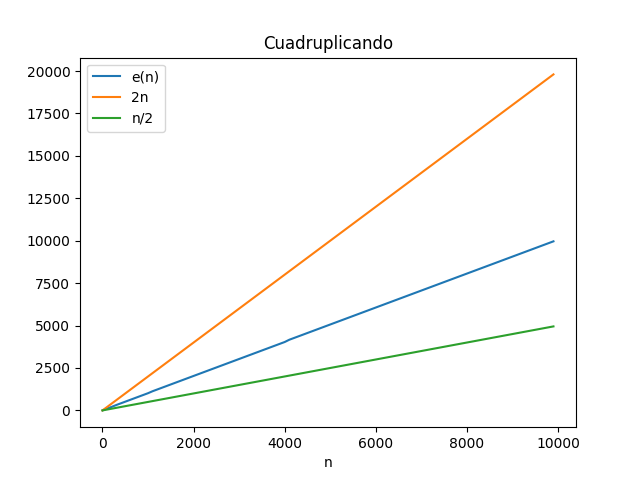
\includegraphics[scale=0.80]{Images/Cuadruplicando.png}
				\end{center}
			\end{figure}

        \end{enumerate}

		Cabe mencionar que el aumentar la cantidad de espacio que se reserva cada vez que el vector se quede sin memoria para almacenar apartir del doble del tamaño de este no será optimo en cuanto a memoria, a pesar de que esto reduce la cantidad de copias que tendremos que hacer de todas formas tenemos que escribir en memoria cada uno de los elementos ingresados al vector por lo que tenemos que hacer al menos $N$ escrituras, pero si incrementa la cantidad de memoria reservada.

		\newpage

		\item  \textbf{(6 puntos: 3 de implementación, 3 de análisis).} Implemente un árbol binario de búsqueda, sin balancear, que permita insertar números enteros. Realice N operaciones de inserción, insertando números en el rango $\bracs{1, 10^{18}}$ generados de forma aleatoria. Si el número ya estaba insertado, no lo reinserte.
		
		\begin{enumerate}
			\item Determine, para el caso peor, cuál es el número de comparaciones entre números llevadas a cabo y expréselo usando notación $\theta$. El número de comparaciones se refiere al total después de la $N$ inserciones. No hace falta demostrar.
			
			El peor caso es cuando ingresas los datos ordenados de mayor a menor o de menor a mayor, ya que así para cada inserción se aumentará en uno el alto del arbol, y el número de comparaciones esta dado por $\theta(N^2)$.

			\item De forma experimental, cuente cuántas comparaciones se hace y grafíquelo para valores de $N$ hasta $10^{8}$. Nótese que dependerá de los valores aleatorios generados, así que ejecútelo varias veces y analice los datos en la forma que considere más oportuna. Encuentre una función que se ajuste de forma adecuada a los datos generados, y trate de explicar qué es lo que está ocurriendo, apoyándose de medidas experimentales sobre el árbol que se está generando, describiendo su intuición sobre lo que está ocurriendo e incluyendo fórmulas que apoyen a su intuición.
			
			Notemos que la altura mínima del BST puede tener es $\ceil{\log_2(n)}$ cuando este es un árbol completo, y su máximo es cuando todo nodo tiene a lo más un hijo donde su altura $h = n$, es decir $\ceil{\log_2(n)} \leq h \leq n$. Son poco los casos que necesitaran hacer un número de comparaciones muy cercano al del peor caso, puesto que la cantidad de vectores de entrada cuyos datos son ordenados (de mayor a menor, o de menor a mayor) son pocos con respecto a la cantidad de vectores posibles, ya que las entradas fueron generadas con $grand()$ (que trata de simular una distribución uniforme entre tmin y tmax). Ahora nos interesaría saber como están dsitribuidas la cantidad de vectores que les toman $k$ comparaciones generar el BST, y ver en donde están mas condensadas para saber que es lo más probable que tome en construir nuestro BST. Por lo datos obtenidos podemos ver que los vectores generados hacen cerca de $nlog(n)$ comparaciones, esta medida se uso puesto que por como se generaron los datos es muy posible que la altura del arbol este más cerca de $\ceil{\log_2(n)}$ que de $n$. Nota para las Comparaciones I/D solo se tomo en cuenta la comparación para encontrar de que lado se inserta el nuevo nodo, en cambio en totales se conto cuando se regunta si ya estaba el valor y/o si ya llegaste al destino de este.

			\begin{figure}[H]
				\begin{center}
					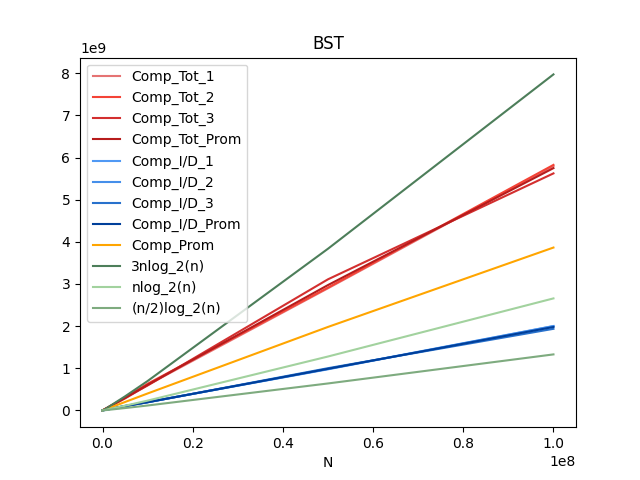
\includegraphics[scale = 0.6]{Images/BST.png}
				\end{center}
			\end{figure}

		\end{enumerate}
		
		\item \textbf{(2 puntos).} Demuestre por reducción al absurdo que para todo entero $k\geq1$, $n^{k-1} = o\pars{n^{k}}$.
		
		\begin{proof}
			Supongamos que para todo $c>0$ existe un $N$ tal que para todo $n \geq N$ se cumple que $n^{k-1} \leq c n^k$, en especial $\frac{1}{N} \leq c$, lo cual es una contradicción puesto que $c$ es un Real y para propiedad arquimediana o completitud de estos siempre habra un número $c$ tal que $0\leq c \leq\frac{1}{0}$.
		\end{proof}
		
    \end{enumerate}
\end{document}

